% !TeX program = xelatex
\documentclass[12pt,a4paper]{ctexart}
\usepackage{amsfonts,amsmath,amssymb,amsthm,graphicx,url}
\usepackage{fullpage}
\usepackage{tikz}
\usetikzlibrary{automata,positioning,arrows.meta,shapes}
\usepackage{enumitem}
\setlist[enumerate]{font=\bfseries}


% Old Stuff
%%\oddsidemargin=0.15in
%%\evensidemargin=0.15in
%%\topmargin=-.5in
%%\textheight=9in
%%\textwidth=6.25in

\setlength{\oddsidemargin}{.1in}
\setlength{\evensidemargin}{.1in}
\setlength{\topmargin}{-0.4in}
\def\eps{\varepsilon}
\def\a{\texttt{a}}
\def\b{\texttt{b}}
\def\ling{\texttt{0}}
\def\yi{\texttt{1}}

\newcommand{\heading}[5]{
   \renewcommand{\thepage}{\arabic{page}}
   \noindent
   \begin{center}
   \framebox{
      \vbox{
    \hbox to 6.2in { {\bf B62005Y-02 理论计算机科学基础}
     	 \hfill #2 }
       \vspace{4mm}
       \hbox to 6.2in { {\Large \hfill #5  \hfill} }
       \vspace{2mm}
       \hbox to 6.2in { {\it #3 \hfill #4} }
      }
   }
   \end{center}
   \vspace*{4mm}
}

\newcommand{\handout}[3]{\heading{#1}{#2}{Instructor: 杨光}{张远航 \textsc{2015K8009929045}}{#3}}

\setlength{\parindent}{0in}
\setlength{\parskip}{0.1in}

\begin{document}
\handout{2}{2017年3月15日}{Solutions to Homework \# 1}

\begin{enumerate}
\item[Sipser 1.14](a) \emph{Proof.} Let $M'$ be the \textsf{DFA} $M$ with the accept and nonaccept states swapped. Suppose $M'$ accepts $x$; then running $M'$ on $x$, we end in an accept state of $M'$. On the other hand, if we run $M$ on $x$, we would end in a nonaccept state. Therefore $x\not\in B$. Similarly, if $x$ is not accepted by $M'$, then it would be accepted by $M$. So $M'$ accepts exactly those strings not accepted by $M$, i.e. $M'$ recognizes the complement of $B$. By the arbitrariness of $B$ we conclude that the class of regular languages is closed under complement. \hfill\qed

(b) Let us consider the example $N_1$ in the textbook (Fig.~1.27). We can check that the string \texttt{101} can be simultaneously accepted by $N_1$ and $N_1'$; hence swapping the accept/nonaccept states does not necessarily yield an \textsf{NFA} recognizing the complement of $C$.

However, the class of languages recognized by \textsf{NFA}s is closed under complement. This follows from the conclusion in part (a) and Theorem 1.39, which implies that the class of languages recognized by \textsf{NFA}s is precisely the class of languages recognized by \textsf{DFA}s.
\item[Sipser 1.16]
(b) To construct an equivalent \textsf{DFA} $D$, we first determine $D$'s state set:
\[\{\emptyset,\{1\},\{2\},\{3\},\{1,2\},\{1,3\},\{2,3\},\{1,2,3\}\}.\]
Next, calculate the $\eps$-closures. For each $R\subseteq Q$, 
\[E(R) = \{q\mid q\text{ can be reached from }R\text{ by travelling along 0 or more }\eps\text{ arrows}\,\},\]
\[E(\emptyset) = \emptyset , E(\{1\}) = \{1,2\}, E(\{2\}) = \{2\}, E(\{3\}) = \{3\},\]
\[E(\{1,2\})=\{1,2\},E(\{1,3\}) = \{1,2,3\}, E(\{2,3\}) = \{2,3\}, E(\{1,2,3\}) = \{1,2,3\}.\]
For each $R\in Q'$ and $a\in\Sigma$, $\delta'(R,a)=\bigcup\limits_{r\in R} E(\delta(r,a))$:
\[\delta'(\emptyset ,a) = \delta'(\emptyset ,b) = \emptyset, \]
\[\delta'(\{1\} ,a) = \{3\}, ~ \delta'(\{1\} ,b) = \emptyset, \]
\[\delta'(\{2\} ,a) = \{1,2\}, ~ \delta'(\{2\} ,b) = \emptyset, \]
\[\delta'(\{3\} ,a) = \{2\}, ~ \delta'(\{3\} ,b) = \{2,3\}, \]
\[\delta'(\{1,2\} ,a) = \{1,2,3\}, ~ \delta'(\{1,2\} ,b) = \emptyset, \]
\[\delta'(\{1,3\} ,a) = \{2,3\}, ~ \delta'(\{1,3\} ,b) = \{2,3\}, \]
\[\delta'(\{2,3\} ,a) = \{1,2\}, ~ \delta'(\{2,3\} ,b) = \{2,3\}, \]
\[\delta'(\{1,2,3\} ,a) = \{1,2,3\}, ~ \delta'(\{1,2,3\} ,b) = \{2,3\}. \]

The new start and accept states are:
\[q_0'=E(q_0)=E(\{1\})=\{1,2\}, \]
\[F' = \{R\in Q'\mid R\text{ contains an accept state of }N\,\} = \{\{2\}, \{1,2\}, \{2,3\}, \{1,2,3\}\}.\]
The \textsf{DFA} $D$ we obtain is shown in the following figure. (The minimal \textsf{DFA} $D_{\min}$ is $D$ with the dashed states and transitions removed.)

\begin{center}
\begin{tikzpicture}[>={Stealth[width=6pt,length=9pt]}, accepting/.style={double distance = 2pt, outer sep = 1pt + \pgflinewidth}, shorten >=1pt, auto]
\draw (100.0pt, -100.0pt)node[state](0){$\emptyset$};
\draw (200.0pt, -100.0pt)node[state,dashed](1){$\{1\}$};
\draw (300.0pt, -100.0pt)node[state,accepting,dashed](2){$\{2\}$};
\draw (400.0pt, -100.0pt)node[state,dashed](3){$\{3\}$};
\draw (100.0pt, -200.0pt)node[state,initial,initial text = ,accepting,ellipse](4){$\{1,2\}$};
\draw (200.0pt, -200.0pt)node[state,ellipse,dashed](5){$\{1,3\}$};
\draw (300.0pt, -200.0pt)node[state,accepting,ellipse](6){$\{2,3\}$};
\draw (400.0pt, -200.0pt)node[state,accepting,ellipse](7){$\{1,2,3\}$};
\path[->] (0) edge[loop above] node{\a, \b}(0);
\path[->] (7) edge[loop below] node{\a}(7);
\path[->] (6) edge[loop above] node{\b}(6);
\path[->] (5) edge[dashed] node{\a, \b}(6);
\path[->] (4) edge[bend right = 30] node{\a}(7);
\path[->] (4) edge node{\b}(0);
\path[->] (2) edge[dashed,bend left = 20] node{\b}(0);
\path[->] (3) edge[dashed] node{\b}(6);
\path[->] (3) edge[dashed] node{\a}(2);
\path[->] (1) edge[bend left = 20,dashed] node{\a}(3);
\path[->] (2) edge[dashed] node{\a}(4);
\path[->] (1) edge[dashed] node{\b}(0);
\path[->] (6) edge[bend left = 20] node{\a}(4);
\path[->] (7) edge node{\b}(6);
\end{tikzpicture}
\end{center}

\item[Sipser 1.21]
(b) The answer is not unique; for example, these expressions are equally valid:
\begin{itemize}
	\item $\mathtt{((a \cup b)a^*b(ba^*b)^*a)^*(\eps \cup ((a \cup b)a^*b(ba^*b)^*))}$,
	% With JFLAP
	\item $\mathtt{((a\cup b)a^*bba^*a)^*((a\cup b)ba^*b\cup\eps)}$,
	% With solnHW3.pdf
	\item $\mathtt{\eps\cup((a\cup b)a^*b((a(a\cup b)\cup b)a^*b)^*(\eps\cup a))}$,
	% With hwSol-5.pdf; add illustration here
	\item $\mathtt{((a\cup b)(a\cup bb)^*ab)^*(\eps \cup (a\cup b)(a\cup bb)^*(b\cup ab))}$.
	% With solnHW3.pdf
\end{itemize}
We give a detailed construction for the third representation:

1. Add a new start state and accept state and necessary $\eps$-transitions; make original final states non-final.

\begin{center}
	\begin{tikzpicture}[>={Stealth[width=6pt,length=9pt]}, accepting/.style={double distance = 2pt, outer sep = 1pt + \pgflinewidth}, shorten >=1pt, auto]
\draw (100.0pt, 0.0pt)node[state, initial, initial text =](0){$q_{\mathrm{start}}$};
\draw (200.0pt, 0.0pt)node[state](1){$1$};
\draw (300.0pt, 0.0pt)node[state](2){$2$};
\draw (150.0pt, -90.0pt)node[state, accepting](3){$q_{\mathrm{accept}}$};
\draw (250.0pt, -90.0pt)node[state](4){$3$};
\path[->] (2) edge[loop right] node{\a}(2);
\path[->] (0) edge node{$\eps$}(1);
\path[->] (4) edge node{\a}(1);
\path[->] (1) edge node{$\eps$}(3);
\path[->] (1) edge node{\a,\b}(2);
\path[->] (4) edge node{$\eps$}(3);
\path[->] (2) edge[bend left = 20] node{\b}(4);
\path[->] (4) edge[bend left = 20] node{\b}(2);
\end{tikzpicture}
\end{center}

2. Perform union on the edge from state $1$ to state $2$.

\begin{center}
	\begin{tikzpicture}[>={Stealth[width=6pt,length=9pt]}, accepting/.style={double distance = 2pt, outer sep = 1pt + \pgflinewidth}, shorten >=1pt, auto]
	\draw (100.0pt, 0.0pt)node[state, initial, initial text =](0){$q_{\mathrm{start}}$};
	\draw (200.0pt, 0.0pt)node[state](1){$1$};
	\draw (300.0pt, 0.0pt)node[state](2){$2$};
	\draw (150.0pt, -90.0pt)node[state, accepting](3){$q_{\mathrm{accept}}$};
	\draw (250.0pt, -90.0pt)node[state](4){$3$};
	\path[->] (2) edge[loop right] node{\a}(2);
	\path[->] (0) edge node{$\eps$}(1);
	\path[->] (4) edge node{\a}(1);
	\path[->] (1) edge node{$\eps$}(3);
	\path[->] (1) edge node{$\a\cup\b$}(2);
	\path[->] (4) edge node{$\eps$}(3);
	\path[->] (2) edge[bend left = 20] node{\b}(4);
	\path[->] (4) edge[bend left = 20] node{\b}(2);
	\end{tikzpicture}
\end{center}

3. Remove state $1$.
\begin{center}
	\begin{tikzpicture}[>={Stealth[width=6pt,length=9pt]}, accepting/.style={double distance = 2pt, outer sep = 1pt + \pgflinewidth}, shorten >=1pt, auto]
	\draw (100.0pt, 0.0pt)node[state, initial, initial text =](0){$q_{\mathrm{start}}$};
	\draw (300.0pt, 0.0pt)node[state](2){$2$};
	\draw (150.0pt, -90.0pt)node[state, accepting](3){$q_{\mathrm{accept}}$};
	\draw (250.0pt, -90.0pt)node[state](4){$3$};
	\path[->] (2) edge[loop right] node{\a}(2);
	\path[->] (0) edge node{$\a\cup\b$}(2);
	\path[->] (4) edge node{$\eps,\a$}(3);
	\path[->] (0) edge node{$\eps$}(3);
	\path[->] (2) edge[bend left = 20] node{\b}(4);
	\path[->] (4) edge[bend left = 20] node{$\a(\a\cup\b),\b$}(2);
	\end{tikzpicture}
\end{center}

4. Perform union on edges.
\begin{center}
	\begin{tikzpicture}[>={Stealth[width=6pt,length=9pt]}, accepting/.style={double distance = 2pt, outer sep = 1pt + \pgflinewidth}, shorten >=1pt, auto]
	\draw (100.0pt, 0.0pt)node[state, initial, initial text =](0){$q_{\mathrm{start}}$};
	\draw (300.0pt, 0.0pt)node[state](2){$2$};
	\draw (150.0pt, -90.0pt)node[state, accepting](3){$q_{\mathrm{accept}}$};
	\draw (250.0pt, -90.0pt)node[state](4){$3$};
	\path[->] (2) edge[loop right] node{\a}(2);
	\path[->] (0) edge node{$\a\cup\b$}(2);
	\path[->] (4) edge node{$\eps\cup\a$}(3);
	\path[->] (0) edge node{$\eps$}(3);
	\path[->] (2) edge[bend left = 20] node{\b}(4);
	\path[->] (4) edge[bend left = 20] node{$\a(\a\cup\b)\cup\b$}(2);
	\end{tikzpicture}
\end{center}

5. Remove state $2$.
\begin{center}
	\begin{tikzpicture}[>={Stealth[width=6pt,length=9pt]}, accepting/.style={double distance = 2pt, outer sep = 1pt + \pgflinewidth}, shorten >=1pt, auto]
	\draw (100.0pt, 0.0pt)node[state, initial, initial text =](0){$q_{\mathrm{start}}$};
	\draw (150.0pt, -90.0pt)node[state, accepting](3){$q_{\mathrm{accept}}$};
	\draw (250.0pt, -90.0pt)node[state](4){$3$};
	\path[->] (4) edge node{$\eps\cup\a$}(3);
	\path[->] (0) edge node{$\eps$}(3);
	\path[->] (0) edge node{$(\a\cup\b)\a^*\b$}(4);
	\path[->] (4) edge[loop right] node{$(\a(\a\cup\b)\cup\b)\a^*\b$}(4);
	\end{tikzpicture}
\end{center}

6. Remove state $3$.
\begin{center}
	\begin{tikzpicture}[>={Stealth[width=6pt,length=9pt]}, accepting/.style={double distance = 2pt, outer sep = 1pt + \pgflinewidth}, shorten >=1pt, auto]
	\draw (0.0pt, 0.0pt)node[state, initial, initial text =](0){$q_{\mathrm{start}}$};
	\draw (300.0pt, 0.0pt)node[state, accepting](3){$q_{\mathrm{accept}}$};
	\path[->] (0) edge node{$\mathtt{\eps,(a\cup b)a^*b((a(a\cup b)\cup b)a^*b)^*(\eps\cup a)}$}(3);
	\end{tikzpicture}
\end{center}

7. Perform union on edges.
\begin{center}
	\begin{tikzpicture}[>={Stealth[width=6pt,length=9pt]}, accepting/.style={double distance = 2pt, outer sep = 1pt + \pgflinewidth}, shorten >=1pt, auto]
	\draw (0.0pt, 0.0pt)node[state, initial, initial text =](0){$q_{\mathrm{start}}$};
	\draw (300.0pt, 0.0pt)node[state, accepting](3){$q_{\mathrm{accept}}$};
	\path[->] (0) edge node{$\mathtt{\eps\cup((a\cup b)a^*b((a(a\cup b)\cup b)a^*b)^*(\eps\cup a))}$}(3);
	\end{tikzpicture}
\end{center}
\item[Sipser 1.28]
(a) The \textsf{NFA} is as follows:
\begin{figure*}[htbp]
	\centering
	\resizebox{0.95\textwidth}{!}{ 
	\begin{tikzpicture}[>={Stealth[width=6pt,length=9pt]}, accepting/.style={double distance = 2pt, outer sep = 1pt + \pgflinewidth}, shorten >=1pt, auto]
\draw (55.0pt, -150.0pt)node[state, initial, initial text =](0){$q_{0}$};
\draw (110.0pt, -120.0pt)node[state](1){$q_{1}$};
\draw (165.0pt, -120.0pt)node[state, accepting](2){$q_{2}$};
\draw (220.0pt, -120.0pt)node[state](3){$q_{3}$};
\draw (275.0pt, -120.0pt)node[state](4){$q_{4}$};
\draw (330.0pt, -120.0pt)node[state](5){$q_{5}$};
\draw (385.0pt, -120.0pt)node[state](6){$q_{6}$};
\draw (440.0pt, -120.0pt)node[state](7){$q_{7}$};
\draw (495.0pt, -120.0pt)node[state, accepting](8){$q_{8}$};
\draw (110.0pt, -190.0pt)node[state](9){$q_{9}$};
\draw (165.0pt, -190.0pt)node[state, accepting](10){$q_{10}$};
\path[->] (9) edge node{\b}(10);
\path[->] (5) edge node{\b}(6);
\path[->] (6) edge node{$\eps$}(7);
\path[->] (0) edge node{$\eps$}(9);
\path[->] (1) edge node{\a}(2);
\path[->] (4) edge node{$\eps$}(5);
\path[->] (7) edge node{\b}(8);
\path[->] (8) edge[bend left = 30] node{$\eps$}(3);
\path[->] (0) edge node{$\eps$}(1);
\path[->] (2) edge node{$\eps$}(3);
\path[->] (3) edge node{\a}(4);
\end{tikzpicture}}
\end{figure*}
\item[Sipser 1.46]\footnote{These questions are labeled as Problem 1.51, 1.68, and 1.73 in the Chinese version of the book.}(c) Suppose that the language $L = \{w\mid w\in\{\ling,\yi\}^*\text{ is not a palindrome}\, \}$ is regular, then $\bar{L} = \{w\mid w\in\{\ling,\yi\}^*\text{ is a palindrome}\, \}$ must be regular. Let $p$ be the pumping length for $\bar{L}$; we choose the string $s$ to be $\ling^p\yi\ling^p$, then the pumping lemma implies that $s = xyz$ with $|y|>0$ and $|xy|\le p$, which means that $y = \ling^k$, where $1\le k\le p$. Since $p-k < p$, $xy^0z=\ling^{p-k}\yi\ling^p$ cannot be in the language $\bar{L}$, a contradiction. Therefore $L$ is not a regular language.\hfill\qed
% From hw2_sol.pdf, solnHW3.pdf
\item[Sisper 1.71](a) Indeed, the language $A$ can be written as the regular expression $\ling (\ling\cup\yi)^*\ling$. First, for each $k\ge 1$, $\ling^ku\ling^k$ is in $\ling (\ling\cup\yi)^*\ling$, so $A\subseteq \ling (\ling\cup\yi)^*\ling$; moreover, for any string $w$ in $\ling (\ling\cup\yi)^*\ling$, $w = \ling^1u\ling^1$, so $\ling (\ling\cup\yi)^*\ling\subseteq A$. Therefore $A = \ling (\ling\cup\yi)^*\ling$.\hfill\qed

(b) Assume that $B$ is a regular language and let $p$ be its pumping length. We choose the string $s$ to be $\ling^p\yi\yi\ling^p$, which is in $B$ and of length $2p+2\ge p$. Thus $s=xyz$ where $|y|>0$ and $|xy|\le p$, which implies that $y=\ling^k$, where $k\ge 1$. Then $xy^2z=\ling^{p+k}\yi\yi\ling^p$ is not in the language $B$, a contradiction. Therefore $B$ is not a regular language.\hfill\qed

\item[Sisper 1.69](b) A string in the language $\overline{WW_k}$ satisfies one of the following conditions:
\begin{itemize}
	\item either $|s|\ne 2k$, or
	\item $s = xy$, where $|x| = |y| = k$ but $x\ne y$.
\end{itemize}
\iffalse
Using the construction given in the proof that ``regular languages are closed under the union (intersection) operation", we can construct several \textsf{NFA}s and combine them into a new machine whose number of states is the product of its components.

First, we can construct an \textsf{NFA} that recognizes $\{s\mid |s|\ne 2k\}$ with $2k$ states; for strings that fall into the second category, there exists some $1\le i\le k$ such that $s_i\ne s_{i+k}$, that is, $s_i = \ling$ and $s_{i+k} = \yi$ or $s_i = \yi$ and $s_{i+k} = \ling$, so $4\sum\limits_{i=1}^k i\cdot (k+i) = O(k^3)$ states are needed. Combining the two categories with the union operation, we obtain an \textsf{NFA} that recognizes $\overline{WW_k}$ with $O(k^4)$ states, which is much smaller than $2^k$ for large $k$'s.
\fi
Therefore we can construct the following \textsf{NFA}:

\begin{figure*}[htbp] 
		\centering 
		\resizebox{0.95\textwidth}{!}{ 
		\begin{tikzpicture}[>={Stealth[width=6pt,length=9pt]}, accepting/.style={double distance = 2pt, outer sep = 1pt + \pgflinewidth}, shorten >=1pt, auto]
		\draw (120.0pt, -270.0pt)node[state, initial, initial text =](0){$q_{0}$};
		\draw (180.0pt, -200.0pt)node[state,accepting](1){$1$};
		\draw (260.0pt, -200.0pt)node[state,accepting](2){$2$};
		\draw (330.0pt, -200.0pt)node(001) {$\ldots\ldots$};
		\draw (400.0pt, -200.0pt)node[state,accepting](3){$2k$};
		\draw (480.0pt, -200.0pt)node[state](4){$2k+1$};
		\draw (560.0pt, -200.0pt)node[state, accepting](5){more};
		\draw (180.0pt, -340.0pt)node[state](6){$q_{1}$};
		\draw (260.0pt, -300.0pt)node[state](7){$q_{2}$};
		\draw (340.0pt, -300.0pt)node[state](8){$1$};
		\draw (410.0pt, -300.0pt)node(002) {$\ldots\ldots$};
		\draw (480.0pt, -300.0pt)node[state](9){$k-1$};
		\draw (560.0pt, -300.0pt)node[state, accepting](10){$k$};
		\draw (260.0pt, -380.0pt)node[state](11){$q_{3}$};
		\draw (340.0pt, -380.0pt)node[state](12){$1$};
		\draw (410.0pt, -380.0pt)node(003) {$\ldots\ldots$};
		\draw (480.0pt, -380.0pt)node[state](13){$k-1$};
		\draw (560.0pt, -380.0pt)node[state, accepting](14){$k$};
		\path[->] (9) edge node{\yi}(10);
		\path[->] (0) edge node{$\eps$}(6);
		\path[->] (1) edge node{\ling,\yi}(2);
		\path[->] (2) edge node{\ling,\yi}(001);
		\path[->] (001) edge node{\ling,\yi}(3);
		\path[->] (8) edge node{\ling,\yi}(002);
		\path[->] (002) edge node{\ling,\yi}(9);
		\path[->] (12) edge node{\ling,\yi}(003);
		\path[->] (003) edge node{\ling,\yi}(13);
		\path[->] (0) edge node{$\eps$}(1);
		\path[->] (5) edge[loop above] node{\ling,\yi}(5);
		\path[->] (7) edge[loop above] node{\ling}(7);
		\path[->] (11) edge[loop below] node{\yi}(11);
		\path[->] (7) edge[bend left] node{\yi}(11);
		\path[->] (11) edge[bend left] node{\ling}(7);
		\path[->] (3) edge node{\ling,\yi}(4);
		\path[->] (13) edge node{\ling}(14);
		\path[->] (6) edge node{\yi}(11);
		\path[->] (7) edge node{\ling,\yi}(8);
		\path[->] (6) edge node{\ling}(7);
		\path[->] (11) edge node{\ling,\yi}(12);
		\path[->] (4) edge node{\ling,\yi}(5);
		\end{tikzpicture}		}
	\end{figure*}
\end{enumerate}

\end{document}
